\documentclass{lab_sheet}
\usepackage{booktabs,caption}
\usepackage[flushleft]{threeparttable}
\usepackage[defernumbers=true,sorting=none]{biblatex}
\DeclareBibliographyCategory{cited}
\AtEveryCitekey{\addtocategory{cited}{\thefield{entrykey}}}
\addbibresource{citation.bib}
\nocite{*} 
\renewcommand*{\thesubfigure}{\thefigure.\arabic{subfigure}}
\newcommand{\digitalpattern}[1]{
    \begin{tabular}{C{2cm}C{1cm}C{1cm}C{1cm}C{1cm}C{1cm}C{1cm}C{1cm}C{1cm}C{2cm}}
        \toprule
          Character & DP & g & f & e & d & c & b & a & HEX value\\
          \midrule
          #1
          \bottomrule
       \end{tabular}
}
\renewcommand{\lstlistlistingname}{Source Codes}
\renewcommand{\lstlistingname}{Code}
\begin{document}
\titlePage{Programming Timers of 8051/8052 Microcontroller}{October 23, 2020}
    \pagenumbering{gobble}
    \tableofcontents
    \pagebreak
    \listoffigures
    \pagebreak
    \listoftables
    \pagebreak
    \lstlistoflistings
    \pagebreak
    \pagenumbering{arabic}
    \section{Introduction}
    \subsection{MCS-51 Family Microcontroller Chips}
    Based on the Harvard architecture of designing ICs, the MCS-51 microcontroller chips were originally developed by Intel to be used in small embedded systems. The MCS-51 chips now use Complementary Metal-Oxide Semiconductor (CMOS) instead of the original NMOS, and are thus known as 80C51 chips. Texas Instruments, Atmel, Dallas Semiconductors, Silicon Laboratories, ASTX, and many more distributors manufacture and sell the MCS-51 family microcontroller chips.\\
    The different features of the 8051 microcontroller are: 
    \begin{itemize}
        \item 8-bit ALU, Accumulator and Registers, making it an 8-bit microcontroller.
        \item 4KB of ROM for the programs, also called program memory.
        \item 8-bit data bus meaning that it can access 8 bits of data in one operation.
        \item 128 Bytes of RAM for the variables, also called data memory.
        \item 32 I/O lines, i.e. 4 ports with 8 lines each.
        \item 16-bit address bus meaning that it can access 65536 locations of RAM and ROM.
        \item 2 16-bit timers/counters.
        \item 1 full-duplex serial port for serial communication (UART).
        \item 6 interrupt sources(2 external interrupts, 2 timer interrupts \& 2 serial interrupts).
        \end{itemize}
        \subsection{Timers in 8051}
        The 8051 microcontroller has two on-chip timers/counters that are used for timing durations for delays or counting external events. Timers allow real-time delays to be implemented in the system. With the frequency at which a microcontroller operates, we can calculate the required delay.\\
        8051 has two timers, namely Timer 0 and Timer 1, which are both 16 bit. Each timer is separated into two bytes namely TH0/TL0 for Timer 0 and TH1/TL1 for Timer 1.
        \subsubsection{TMOD Register}
        \begin{figure}[H]
            \centering
            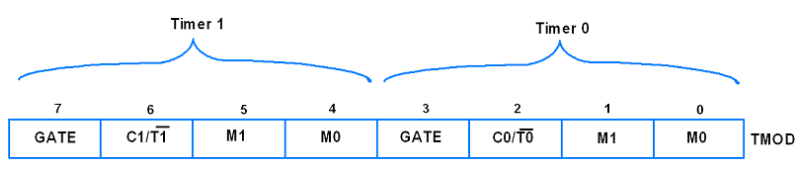
\includegraphics[scale=0.7]{../Figures/tmod}
            \caption{TMOD register bit description}
            \label{fig:tmod}
        \end{figure}
        TMOD is an 8-bit register that is used by both the timers in 8051. The lower nibble is used by Timer 0 and upper nibble is used by Timer 1. Short description for each bit is mentioned below:
        \subsubsection*{Gate}
        Gating control bit is used to select between the timer/counter mode. When set, timer is enable when INTx pin is high and TRx control pin is set. When cleared, timer is enabled TRx control bit is set.
        \subsubsection*{Counter/Timer}
        Cleared to enable timer. Set to enable counter operation.
        \subsubsection*{M1 and M0}
        Used as select pins for different modes of timers.
        \begin{table}[H]
            \centering
            \begin{tabular}{C{2cm}C{2cm}C{2cm}C{6cm}}
            \toprule
              M1 & M0 & Mode & Description\\
              \midrule
              0 & 0 & 0 & 13-bit timer mode: 8-bit timer/counter 8 bit of THx and least significant 5 bits of TLx are cascaded.\\\hline
              0 & 1 & 1 & 16-bit timer mode: 16-bit timer/counter THx and TLx are cascaded.\\\hline
              1 & 0 & 2 & 8-bit auto reload: THx holds a value which is to be reloaded in TLx each time it overflows.\\\hline
              1 & 1 & 3 & Split timer mode: Split 16-bit timerx into two 8-bit timer i.e. THx and TLx like two 8-bit timer.  Only Timer 0 is used in this mode.\\
              \bottomrule
           \end{tabular}
      \caption{Timer modes selection combinations}
      \label{tbl:modes}
        \end{table}
        \subsubsection{TCON Register}
        \begin{figure}[H]
            \centering
            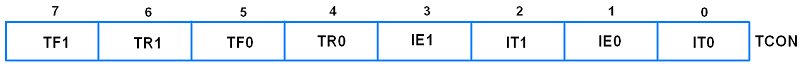
\includegraphics[scale=0.7]{../Figures/tcon}
            \caption{TCON register bit description}
            \label{fig:tcon}
        \end{figure}
        TCON is an 8-bit register used by both timers in 8051 as well as interrupts. THe lower nibble is used by interrupts and upper nibble is used by timers. Short description for each bit is mentioned below:
        \subsubsection*{TF1 and TF0}
        Timer 1 and Timer 0 overflow flags. Set when timer overflows the maximum value.
        \subsubsection*{TR1 and TR0}
        Timer 1 and Timer 0 run enable. Set to start the respective timer, and reset to stop the timer.
        \subsubsection*{IE1 and IE0}
        Interrupt 1 and Interrupt 0 edge detect flags. Set when interrupt edge is detected.
        \subsubsection*{IT1 and IT0}
        Interrupt 1 and Interrupt 0 type control bits. When set, it detects the falling edge interrupt, when cleared it detects zero level interrupt.
        \subsubsection{Timer Modes}
        \subsubsection*{Timer Mode 0 (13-bit timer mode)}
        This mode is selected by choosing M1 = 0 and M0 = 0
in the TMOD register. TH (8-bit) and TL (lower 5 bits) of
timer are cascaded to form a 13-bit timer. Values
from 0000 H to 1FFF H can be loaded into timer’s register.
After loading required values to TH and TL register,
Timer 0 is started using command SETB TR0 and Timer 1
is started by using the command SETB TR1. Timer counts
from loaded values up to 1FFF H and rolls over to 0000 H
setting TF0 flag for Timer 0 and TF1 for Timer 1.
\subsubsection*{Timer Mode 1 (16-bit timer mode)}
This mode is selected by choosing M1 = 0 and M0 = 1
in the TMOD register. TH (8-bit) and TL (8 bits) of timer
are cascaded to form a 16-bit timer. Values from 0000 H
to FFFF H can be loaded into timer’s register. After loading required values to TH and TL register,
Timer 0 is started using command SETB TR0 and Timer 1
is started by using the command SETB TR1. Timer counts
from loaded values up to FFFF H and rolls over to 0000 H
setting TF0 flag for Timer 0 and TF1 for Timer 1. 
\subsubsection*{Timer Mode 2 (8-bit auto reload mode)}
This mode is selected by choosing M1 = 1 and M0 = 0
in the TMOD register. Only TL (8 bits) register of timer is
used. Values from 00 H to FF H can be loaded into timer’s
register. TH register automatically loads a copy of the
initial value into TL register.
After TL receives a copy of the 8-bit initial value, TL0
of Timer 0 is started using command SETB TR0 and TL1
of Timer 1 is started by using the command SETB TR1.
Timer counts from loaded values up to FF H and rolls over
to 00 H setting TF0 flag for Timer 0 and TF1 for Timer 1.
\subsubsection*{Timer Mode 3 (Split timer mode)}
This mode is selected by choosing M1 = 1 and M0 = 1
in the TMOD register. Timer 0 splits into two 8-bit timers.
TL0 and TH0 act as two separate timers. TL0 uses TR0 and
TF0 while TH0 uses TR1 and TF1 bit. After TL0 and/or TH0 are initialized with 8-bit initial
value, timers are started. TL0 is started using command
SETB TR0 and TH0 is started by using the command
SETB TR1. Timer counts from loaded values up to FF H
and rolls over to 00 H setting TF0 flag if TL0 overflows
and setting TF1 flag if TH0 overflows. Only Timer 0 can be used in this mode.
\subsubsection{Delay calculation}
The required timer mode is selected using the combinations mentioned in Table~\ref{tbl:modes}. The timer is clocked by an external oscillator of frequency 11.0592 MHz. The frequency for timer is $(\frac{1}{12})^{th}$ of the frequency of external oscillator.
       \begin{equation*}
        \begin{aligned}
        Frequency~of~oscillator &= 11.0592 MHz\\
        Machine~cycle~frequency &= \frac{11.0592}{12}=921.6~KHz\\
        Machine~cycle~period &= \frac{1}{921.6~KHz}=1.085~\mu s
    \end{aligned}
       \end{equation*} 
        Consider that we want a delay of $T$ seconds. We can calculate the required HEX values to be entered in TH and TL of the timer registers in different modes as,\\
        \begin{equation*}
            \begin{aligned}
            (Z)_{10}&=\frac{T}{1.085~\mu s}\\
            (N)_{10}&=(Maximum~timer~value+1)-Z_{10}
        \end{aligned}
        \end{equation*}
        Converting $(N)_{10}$ into hexadecimal value will give the required hex output that needs to be stored in the THx and/or TLx. It is to be noted that the \textit{maximum timer value} is different for different modes and the final hexadecimal value needs to be cascaded into equivalent form as per the mode.
    \subsection{7-Segment LED Display}
    7-segment LED display is a basic electronic device that is made up of 7 led segments each arranged in such a way that specific configurations of these LEDs allow certain alpha-numeric characters to be displayed on the device. Most 7-segment LEDs also contain an additional LED to indicate the decimal point when two or more 7-segment LED displays are used in conjuction. Each of the seven LEDs have a positional reference with pin outs generally being named as a, b, c, d, e, f, g and DP. One end of all the LEDs are commoned out whereas other end is provided with a proper biasing voltage to either turn on or off the segment depending on the terminal polarity. Forward biasing of the appropriate LED segments are used to display the desired character or pattern. Widely used in digital clocks, small-scale calculators, electronic meters and digital display units, the 7-segment LED displays serve a handy purpose in digital electronics.
    \subsubsection{Digital Drive Pattern}
    For a common cathode 7-segment LED display, the segments a through g and DP must be provided HIGH logic in order to be turned on. Likewise, for a common anode 7-segment LED display, the segments a through g and DP must be provided LOW logic in order to be turned on. The different combinations that are to be used to display certain characters are called digital drive pattern. The table that stores these patterns is called a lookup table.
    \begin{table}[H]
        \centering
        \begin{threeparttable}
        \digitalpattern{0 & 0 & 0 & 1 & 1 & 1 & 1 & 1 & 1 & 3F H\\
        1 & 0 & 0 & 0 & 0 & 0 & 1 & 1 & 0 & 06 H\\
        2 & 0 & 1 & 0 & 1 & 1 & 0 & 1 & 1 & 5B H\\
        3 & 0 & 1 & 0 & 0 & 1 & 1 & 1 & 1 & 4F H\\
        4 & 0 & 1 & 1 & 0 & 0 & 1 & 1 & 0 & 66 H\\
        5 & 0 & 1 & 1 & 0 & 1 & 1 & 0 & 1 & 6D H\\
        6 & 0 & 1 & 1 & 1 & 1 & 1 & 0 & 1 & 7D H\\
        7 & 0 & 0 & 0 & 0 & 0 & 1 & 1 & 1 & 07 H\\
        8 & 0 & 1 & 1 & 1 & 1 & 1 & 1 & 1 & 7F H\\
        9 & 0 & 1 & 1 & 0 & 1 & 1 & 1 & 1 & 6F H\\}
  \begin{tablenotes}
    \small
    \item Note: For displaying any character along with a decimal point, the HEX value should be ORed with 80 H.
  \end{tablenotes}
  \caption{Lookup table for a Common-Cathode 7-segment display}
  \label{tbl:cc}
        \end{threeparttable}
    \end{table}
    \section{Objectives}
    The primary objective of this lab experiment is to understand various programming concepts for timers in 8051/8052 microcontroller. The programming concepts for timers will enable us to write assembly and Embedded C codes for the 8051/8052 microcontroller capable of:
    \begin{itemize}
        \item Applying timers in different timing modes.
        \item Implementing accurate delays using timers.
    \end{itemize}
    \section{Lab Experiment Environment}
    The lab experiments will be performed virtually via various simulation softwares. The basic usages of these tools will allow us to write and visualize different programs involving timers in 8051/8052 microcontroller. Due to a simulated environment, the observations are carefully selected to represent the problems with maximum efficiency.
    \subsection{Circuit Simulation}
    A profession PCB layout, circuit design and simulation tool, Proteus Design Suite was used to simulate the interface between a 8052 microcontroller and an oscilloscope for Problem 1 and Problem 2, and a common cathode 7-segment LED display for Problem 3. Additional electronic components such as resistors, resistor bus, transistors were also used to attain the circuits shown in Figure~\ref{fig:proteus}.
    \begin{figure}[H]
        \begin{subfigure}{.5\textwidth}
            \centering
            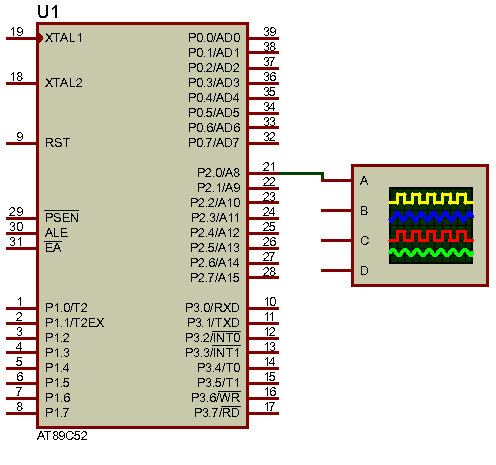
\includegraphics[height=.9\linewidth,width=.9\linewidth]{../Figures/3_1}
            \caption{Schematic for Problem 1}
            \label{fig:proteus_a}
        \end{subfigure}
        \begin{subfigure}{.5\textwidth}
            \centering
            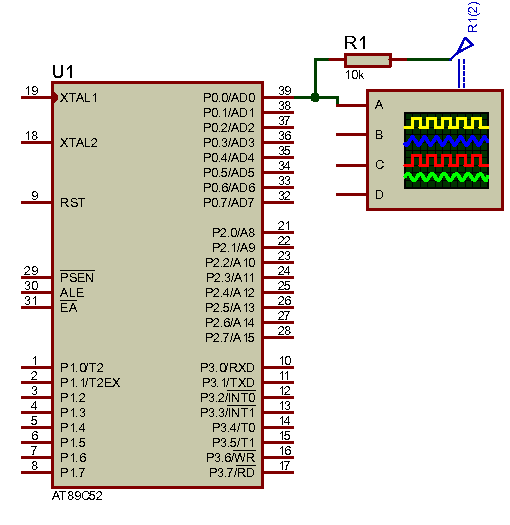
\includegraphics[height=.9\linewidth,width=.9\linewidth]{../Figures/3_2}
            \caption{Schematic for Problem 2}
            \label{fig:proteus_a}
        \end{subfigure}
        \hspace*{\fill}
      \begin{subfigure}{.5\textwidth}
        \centering
        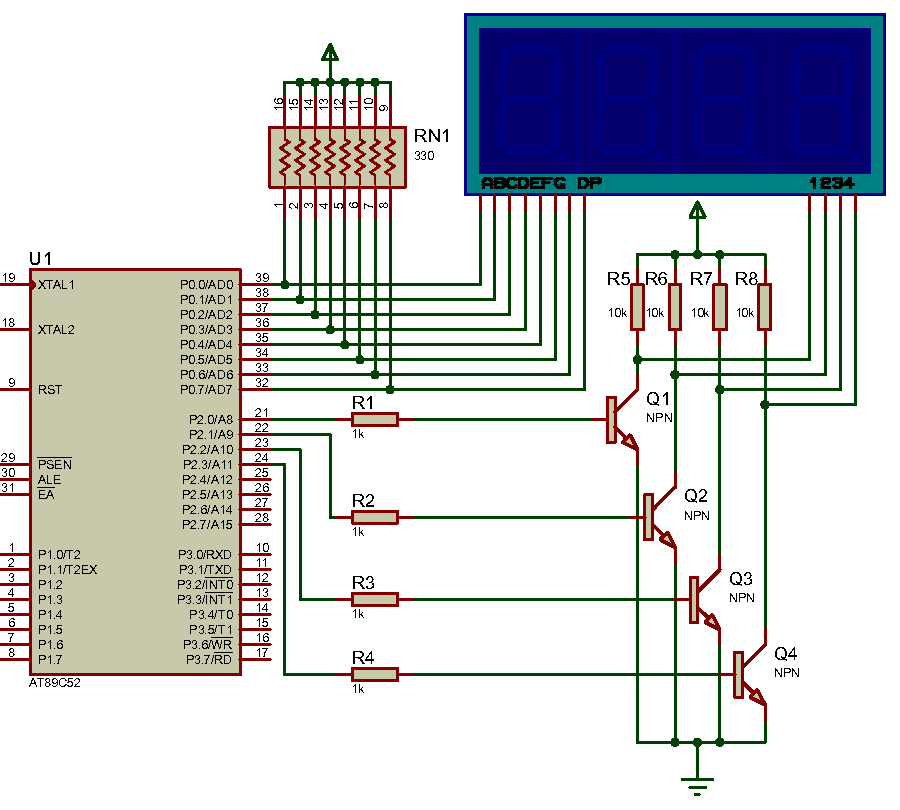
\includegraphics[width=.9\linewidth]{../Figures/3_3}   
        \caption{Schematic for Problem 3}
        \label{fig:prob1-s}
      \end{subfigure}
      \hspace*{\fill}
        \caption{Circuit diagrams for Proteus simulation}
        \label{fig:proteus}
    \end{figure}
    \subsection{Code Editor and Compiler}
    KEIL $\mu$Vision, which is a product of the ARM Ltd. was used as the code editor for the assembly and embeddded C codes for the different lab problems. KEIL products include C/C++ compilers, debuggers, integrated development and simulation environments, RTOS and
    middleware libraries, and evaluation boards for ARM, Cortex-M, Cortex-R4, 8051, C166, and 251 processor families. The compiler built-in with KEIL converts the codes into respective HEX codes that are understandable by the microcontroller.
    \section{Lab Problems}
    \problem{Generate a periodic square wave having a period of 15 ms and a duty cycle of 20\%. The waveform should be produced at pin zero of port two (P2.0). The XTAL frequency is 11.0592 MHz. Observe the waveform on an oscilloscope and measure the ON and OFF timers.}
    \begin{figure}[H]
        \centering
        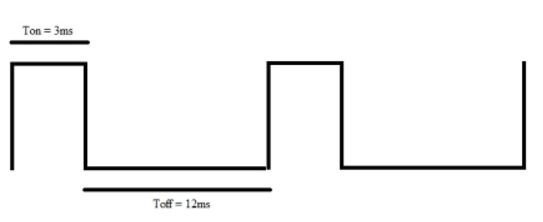
\includegraphics{../Figures/p1}
        \label{fig:p1}
        \caption{Waveform to be generated for Problem 1}
    \end{figure}
    \subproblem{Using Timer 1 in mode 0 (13-bit timer mode)}
    \code{lab3_1_a}
    \subproblem{Using Timer 0 is mode 1 (16-bit timer mode)}
    \code{lab3_1_b}
    \subproblem{Using Timer 1 in mode 2 (8-bit auto-reload timer mode)}
    \code{lab3_1_c}
    \subproblem{Using Timer 0 (TL0) in mode 3 (8-bit split timer mode)
    }
    \code{lab3_1_d}
    \problem{Generate the periodic waveform as shown in figure 11. The waveform should be produced at pin zero of port zero (P0.0). The XTAL frequency is 11.0592 MHz. Observe the waveform on an oscilloscope and measure the ON and OFF times. }
    \begin{figure}[H]
        \centering
        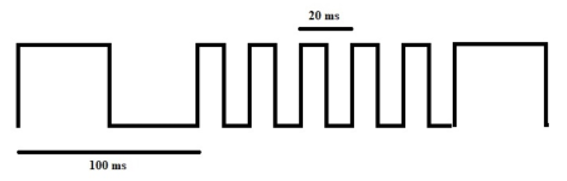
\includegraphics{../Figures/p2}
        \label{fig:p1}
        \caption{Waveform to be generated for Problem 2}
    \end{figure}
    \subproblem{Using Timer 0 in mode 0 (13-bit timer mode)}
    \code{lab3_2_a}
    \subproblem{Using Timer 1 is mode 1 (16-bit timer mode)}
    \code{lab3_2_b}
    \subproblem{Using Timer 0 in mode 2 (8-bit auto-reload timer mode)}
    \code{lab3_2_c}
    \subproblem{Using Timer 0 (TH0) in mode 3 (8-bit split timer mode)
    }
    \code{lab3_2_d}
    \problem{Design a digital minutes and seconds in double digit format. The clock should count from 00:00 to 59:59 and repeat. Time should be displayed in decimal format using four 7-segment LED units. A decimal point should separate minutes from seconds. Use an appropriate timer and timer mode. Use port 0 (P0) to send data to 7-segment LED units. Use transistors as switches to activate or deactivate the 7-segment LED units using pins 0, 1, 2 and 3 of port 2 (P2.0, P2.1, P2.2, P2.3).}
    \code{lab3_3}
    \section{Observations}
    The observations for the oscilloscope observations are taken from Proteus in VSM debugging mode. The different waveforms obtained are better observed with cursors labeling the different time variations at key points. The waveforms as required by the questions are observed in the oscilloscope with minimum variations in the delays. Minor variations in the timing are results of neglected decimal values while calculating delays. For the digital clock as required by Problem 3, the 7-segment display was used. Few snippets of the observed display have been included. It is to be noted that the timings as shown in the observations vary by about 5 ms for 30 minutes run. This is most likely due to the neglected decimal points in delay calculation.
    \subsubsection*{Problem 1}
    \begin{figure}[H]
        \begin{subfigure}{.5\textwidth}
        \centering
        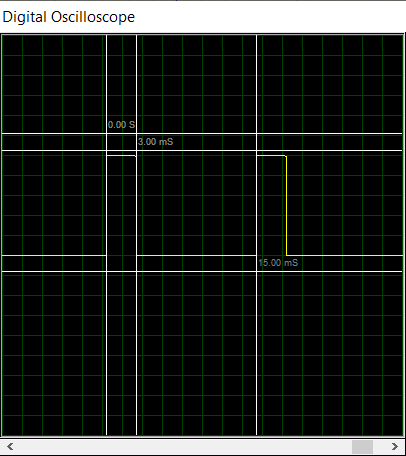
\includegraphics[width=.8\linewidth,frame]{../Figures/1a.png}
        \caption{}
        \label{fig:prob1_a}
        \end{subfigure}
        \begin{subfigure}{.5\textwidth}
            \centering
            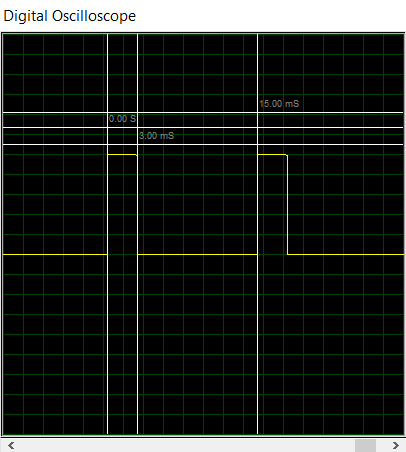
\includegraphics[width=.8\linewidth,frame]{../Figures/1b.png}
            \caption{}
            \label{fig:prob1_b}
            \end{subfigure}
            \newline
            \begin{subfigure}{.5\textwidth}
                \centering
                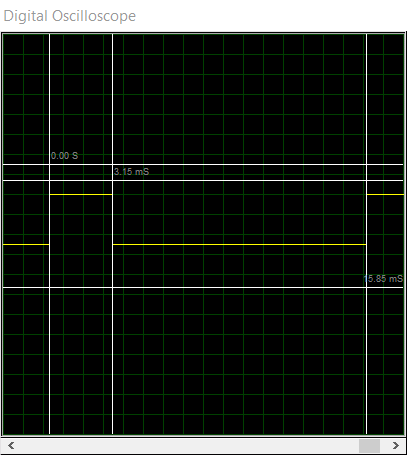
\includegraphics[width=.8\linewidth,frame]{../Figures/1c.png}
                \caption{}
                \label{fig:prob1_c}
                \end{subfigure}
                \begin{subfigure}{.5\textwidth}
                    \centering
                    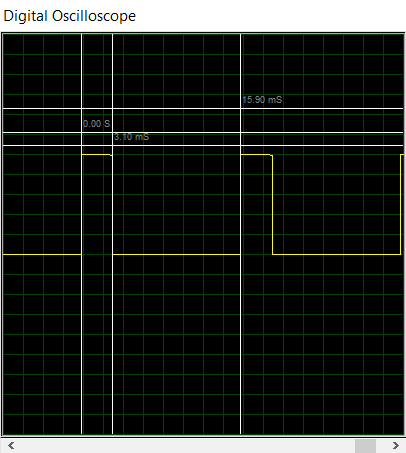
\includegraphics[width=.8\linewidth,frame]{../Figures/1d.png}
                    \caption{}
                    \label{fig:prob1_d}
                    \end{subfigure}
                    \caption{Observation for Problem 1}
                    \label{fig:prob1}
    \end{figure}
    Figure~\ref{fig:prob1} shows the observations for Problem 1. The observations for mode 0 and mode 1 are undeviated from actual requirement but that for mode 2 and mode 3 are slightly off due to error in delay calculation. This can be solved by a detailed analysis of the exact machine cycles needed for the delay to be exact.
    \subsubsection*{Problem 2}
    \begin{figure}[H]
        \begin{subfigure}{.5\textwidth}
        \centering
        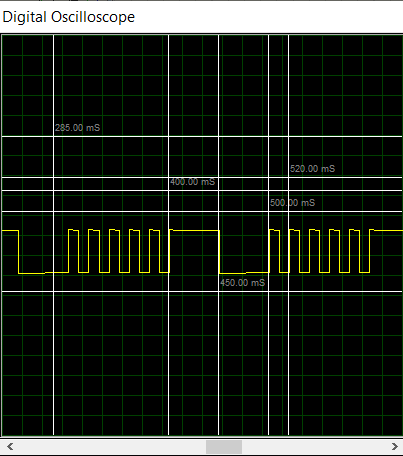
\includegraphics[width=.8\linewidth,frame]{../Figures/2a.png}
        \caption{}
        \label{fig:prob2_a}
        \end{subfigure}
        \begin{subfigure}{.5\textwidth}
            \centering
            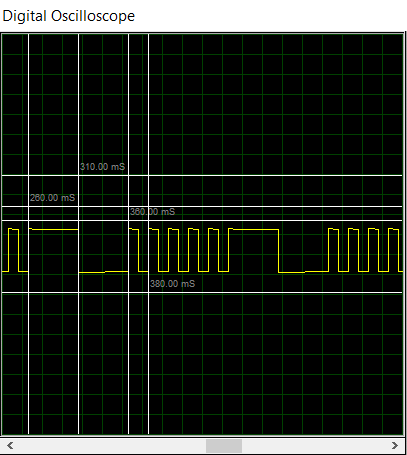
\includegraphics[width=.8\linewidth,frame]{../Figures/2b.png}
            \caption{}
            \label{fig:prob2_b}
            \end{subfigure}
            \newline
            \begin{subfigure}{.5\textwidth}
                \centering
                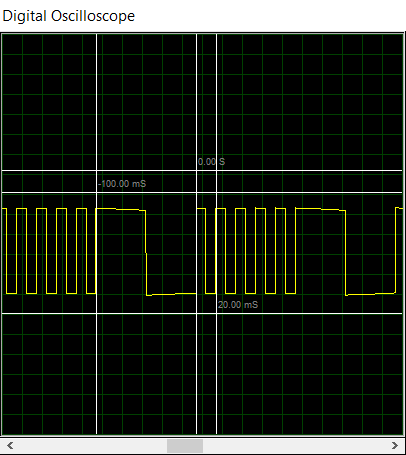
\includegraphics[width=.8\linewidth,frame]{../Figures/2c.png}
                \caption{}
                \label{fig:prob2_c}
                \end{subfigure}
                \begin{subfigure}{.5\textwidth}
                    \centering
                    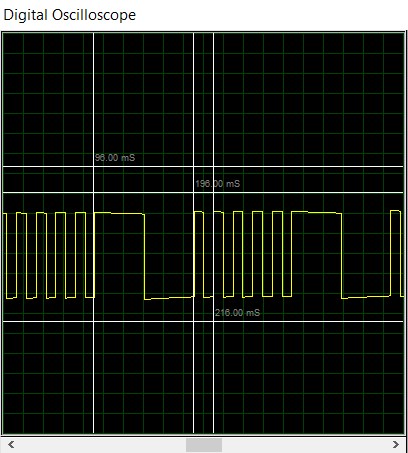
\includegraphics[width=.8\linewidth,frame]{../Figures/2d.png}
                    \caption{}
                    \label{fig:prob2_d}
                    \end{subfigure}
                    \caption{Observation for Problem 2}
                    \label{fig:prob2}
    \end{figure}
    Figure~\ref{fig:prob2} shows the observations for Problem 2. The observations for mode 0, mode 1 and mode 2 are undeviated from actual requirement but that mode 3 is slightly off due to error in delay calculation. This can be solved by a detailed analysis of the exact machine cycles needed for the delay to be exact.
    \subsubsection*{Problem 3}
    \begin{figure}[H]
        \begin{subfigure}{.5\textwidth}
        \centering
        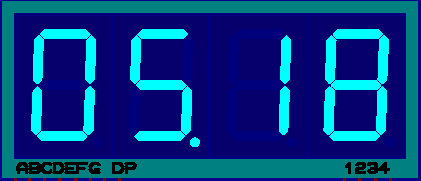
\includegraphics[width=.8\linewidth,frame]{../Figures/3a}
        \caption{}
        \label{fig:prob3_a}
        \end{subfigure}
        \begin{subfigure}{.5\textwidth}
            \centering
            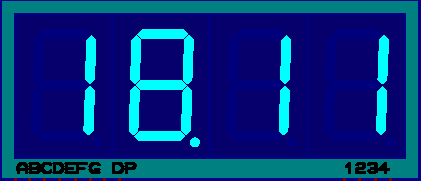
\includegraphics[width=.8\linewidth,frame]{../Figures/3c}
            \caption{}
            \label{fig:prob3_b}
            \end{subfigure}
            \newline
            \begin{subfigure}{.5\textwidth}
                \centering
                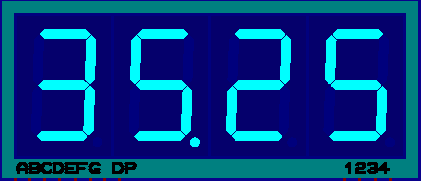
\includegraphics[width=.8\linewidth,frame]{../Figures/3b}
                \caption{}
                \label{fig:prob3_c}
                \end{subfigure}
                \begin{subfigure}{.5\textwidth}
                    \centering
                    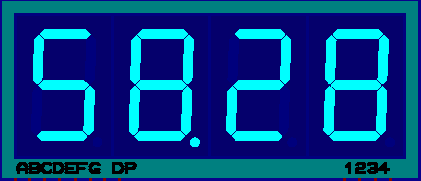
\includegraphics[width=.8\linewidth,frame]{../Figures/3d}
                    \caption{}
                    \label{fig:prob3_d}
                    \end{subfigure}
                    \caption{Observation for Problem 3}
                    \label{fig:prob3}
    \end{figure}
    Figure~\ref{fig:prob3} shows the observations for Problem 3. The digital clock was achieved by introducing accurate delays for a clock to function. 7-segment LED displays were fed with accurate delays between the multiplexed lines to avoid flickering. Port 0 is used to feed the bit configurations for the LED units. Timer mode 1 is used for programming purpose since it is the easiest way to program a delay. The values for minute and second are compared with 60 such that any values crossing it would change either the minute hand or reset the clock as a whole. The minute and second denominations are separated by decimal point by ORing the minute's ones place value. The simulation results for four different points of time are shown above and the results were cross checked with the Proteus VSM animating clock which is considered to be real-time.
    \section{Discussion}
    In this lab experiment, programming timers in 8051/8052 was dealt with various problems at hand. Various waveforms with varying delays were produced using ports of an 8051/8052 microcrontroller by using delays from timers. Different modes of timers were practiced, and it helped us attain much needed programming concepts for timers in 8051 using both assembly and Embedded C langugaes.
    \pagebreak
    \printbibliography[heading=bibintoc,title={Additional References},notcategory=cited]
\end{document}